\documentclass[xcolor=dvipsnames]{beamer}
%\documentclass[xcolor=dvipsnames,handout]{beamer}


\usepackage{animate}
%\usepackage{pgfpages}
%\setbeameroption{second mode text on second screen=left}
%\usepackage{CJK}
%\usepackage{ctex}
\usepackage[english]{babel}
%\usepackage[latin1]{inputenc}
\usepackage{graphicx}
\usepackage{bm}
\usepackage{textpos}
\usepackage{algpseudocode}
\usepackage{algorithm}
\usepackage[caption=false]{subfig}
\usepackage{stfloats}
\usepackage{url}
\usepackage{multirow}
\usepackage{threeparttable}
\usepackage{bookmark}
\usepackage{times}
\usepackage[T1]{fontenc}
\usepackage{ulem,tikz}
\usetikzlibrary{arrows}
\tikzstyle{block}=[draw opacity=0.7,line width=1.4cm]
%\usepackage[bottom]{footmisc}
\usepackage{multimedia}
\captionsetup{font=scriptsize,labelfont=scriptsize}
\hypersetup{pdfpagemode=UseNone}

% Define code layout to insert code
\usepackage{listings}
\usepackage{color}
\lstset{
		language=[GNU]C++,
		basicstyle=\scriptsize,
		breaklines=false,
		xleftmargin=.2in,
		xrightmargin=.2in,
		prebreak=\raisebox{0ex}[0ex][0ex]{\ensuremath{\hookleftarrow}},
		frame=lines,
		shwotabs=false,
		showspaces=false,
		showstringspaces=false,
		extendedchars=true,
		identifierstyle=\ttfamily,
		keywordstyle=\color{blue!50!red}\bfseries,
		commentstyle=\color{green!50!black}\itshape,
		stringstyle=\color{blue},
		numbers=left,
		numbersep=5pt,
		numberstyle=\tiny,
		captionpos=t,
		escapeinside={\%*}{*)}
	   }

% Set citations
\usepackage{csquotes}
%\usepackage[style=numeric-comp,autocite=footnote,citetracker=true,maxnames=1,sorting=none,babel=hyphen,hyperref=true,backend=biber]{biblatex}
\usepackage[style=numeric-comp,autocite=footnote,citetracker=true,maxnames=1,sorting=none]{biblatex}
%\usepackage[style=verbose,autocite=footnote,citetracker=true,maxnames=1,sorting=none,babel=hyphen,hyperref=true,backend=biber]{biblatex}
%\setbeamersize{text margin left=8pt,text margin right=8pt}

%\setlength{\skip\footins}{25cm plus 0cm minus 25cm}
%\setlength{\footnotesep}{0.3cm}
%\renewcommand*{\bibfont}{\tiny}

\setbeamertemplate{bibliography item}{%
  \ifboolexpr{ test {\ifentrytype{book}} or test {\ifentrytype{mvbook}}
    or test {\ifentrytype{collection}} or test {\ifentrytype{mvcollection}}
    or test {\ifentrytype{reference}} or test {\ifentrytype{mvreference}} }
    {\setbeamertemplate{bibliography item}[book]}
    {\ifentrytype{online}
       {\setbeamertemplate{bibliography item}[online]}
       {\setbeamertemplate{bibliography item}[article]}}%
  \usebeamertemplate{bibliography item}}

\defbibenvironment{bibliography}
  {\list{}
     {\settowidth{\labelwidth}{\usebeamertemplate{bibliography item}}%
      \setlength{\leftmargin}{\labelwidth}%
      \setlength{\labelsep}{\biblabelsep}%
      \addtolength{\leftmargin}{\labelsep}%
      \setlength{\itemsep}{\bibitemsep}%
      \setlength{\parsep}{\bibparsep}}}
  {\endlist}
  {\item}

% Settings for footnote and citation
\DeclareCiteCommand{\footfullcitetext}
  [\let\thefootnote\relax\mkbibfootnotetext]
  {\usebibmacro{prenote}}
  {\mkbibbrackets{\thefield{labelnumber}}%
   \addnbspace
   \usedriver
     {\DeclareNameAlias{sortname}{default}}
     {\thefield{entrytype}}}
  {\multicitedelim}
  {\usebibmacro{postnote}}

\makeatletter

%% this stuff fixes the frame numbering in beamer when using an appendix such
%% that the slides of the appendix are not counted in the total framenumber
\let\appendixtotalframenumber\empty
\def\mainend{-1}
\let\appendixorig\appendix

\def\appendix{
  \edef\mainend{\theframenumber}
  \immediate\write\@auxout{\string\global\string\@namedef{mainendframenumber}{\mainend}}
  \appendixorig
  \def\inserttotalframenumber{\appendixtotalframenumber}%
  \setcounter{framenumber}{0}
}

\def\pageatend{
  \edef\appendixend{\theframenumber}
  \ifnum\mainend>0%
  \immediate\write\@auxout{\string\global\string\@namedef{appendixtotalframenumber}{\appendixend}}%
  \immediate\write\@auxout{\string\global\string\@namedef{inserttotalframenumber}{\mainend}}%
  \immediate\write\@auxout{\string\@writefile{nav}{\noexpand \headcommand {%
        \noexpand \def\noexpand \inserttotalframenumber{\mainend}}}}%
  \immediate\write\@auxout{\string\@writefile{nav}{\noexpand \headcommand {%
        \noexpand \def\noexpand \appendixtotalframenumber{\appendixend}}}}%
  \else
  \fi
}

\AtEndDocument{\pageatend}

% Define footnote for block
\let\cbx@citehook=\empty
\newtoggle{cbx@blockcite}

\renewcommand{\@makefntext}[1]{%
  \noindent\normalfont\@thefnmark#1}

\DeclareCiteCommand{\sfcite}[\cbx@superscript]%
  {\usebibmacro{cite:init}%
   \let\multicitedelim=\supercitedelim
   \iffieldundef{prenote}{}{\BibliographyWarning{Ignoring prenote argument}}%
   \iffieldundef{postnote}{}{\BibliographyWarning{Ignoring postnote argument}}}
  {\usebibmacro{citeindex}%
   \ifciteseen
     {\ifnumequal{\value{page}}{\csuse{cbx@page@\thefield{entrykey}}}
       {}
       {\ifnumequal{\value{framenumber}}{\csuse{cbx@frame@\thefield{entrykey}}}
          {\usebibmacro{sfcite}}
          {}}}
     {\usebibmacro{sfcite}}%
   \usebibmacro{cite:comp}}
  {}
  {\usebibmacro{cite:dump}}

\newbibmacro*{sfcite}{%
  \csnumgdef{cbx@page@\thefield{entrykey}}{\value{page}}%
  \csnumgdef{cbx@frame@\thefield{entrykey}}{\value{framenumber}}%
  \xappto\cbx@citehook{%
    \noexpand\footfullcitetext{\thefield{entrykey}}}}

\newrobustcmd*{\cbx@superscript}[1]{%
  \mkbibsuperscript{\mkbibbrackets{#1}}%
  \iftoggle{cbx@blockcite}
    {}
    {\cbx@citehook%
     \global\let\cbx@citehook=\empty}}

\BeforeBeginEnvironment{block}{\global\toggletrue{cbx@blockcite}}

\def\metabox#1{\edef\theprevdepth{\the\prevdepth}\nointerlineskip
  \vbox to0pt{#1\vss}\prevdepth=\theprevdepth}

\AfterEndEnvironment{block}
  {\metabox{%
     \global\togglefalse{cbx@blockcite}%
     \cbx@citehook%
     \global\let\cbx@citehook=\empty}}


\BeforeBeginEnvironment{exampleblock}{\global\toggletrue{cbx@blockcite}}

\def\metabox#1{\edef\theprevdepth{\the\prevdepth}\nointerlineskip
  \vbox to0pt{#1\vss}\prevdepth=\theprevdepth}

\AfterEndEnvironment{exampleblock}
  {\metabox{%
     \global\togglefalse{cbx@blockcite}%
     \cbx@citehook%
     \global\let\cbx@citehook=\empty}}

\AtEveryCitekey{\iffootnote{\tiny}{\color{blue}}{\vspace{-1ex}}}
\renewcommand*{\footnoterule}{\kern -1pt \hrule \@width 2in \kern 1pt}

\makeatother


\mode<presentation>
{
  \usetheme{CambridgeUS} % Show Section/Subsection on header
  %\usetheme{Boadilla}
  %\usetheme{Madrid}     % Show no Section/Subsection on header

  %\usefonttheme{structurebold}
  %\usecolortheme{dolphin}
  \usecolortheme{seahorse}

  \useinnertheme{circles}
  %\useoutertheme{default}
  %\useoutertheme{infolines}

  %\useoutertheme{split}

  \usecolortheme[named=OliveGreen]{structure}

  %Header, navigation and footer
  \setbeamertemplate{navigation symbols}{}
  \setbeamertemplate{footline}[frame number]
  \setbeamercolor{page number in head/foot}{fg=black}
  \setbeamercolor{title}{fg=black}
  \setbeamerfont{frame number}{family=\bf}
  %\setbeamercovered{transparent}
  %\setbeamertemplate{sidebar left}{}% or get rid of navigation entries there somehow
  %\addtobeamertemplate{footline}{\hfill\usebeamertemplate***{navigation symbols}\par}{}
}
%\setbeameroption{show notes on second screen}
%\setbeamertemplate{note page}[compress]
\setbeamertemplate{caption}[numbered]
\setbeamerfont{caption}{size=\scriptsize}
\setbeamercovered{invisible}

\addbibresource{Bib.bib}

\title[Beamer Template] % (optional, use only with long paper titles)
{Beamer Template}

\author[Yongsen Ma] % (optional, use only with lots of authors)
{Yongsen Ma}
% - Give the names in the same order as the appear in the paper.
% - Use the \inst{?} command only if the authors have different
%   affiliation.

\institute[William \& Mary] % (optional, but mostly needed)
{
  %The College of William and Mary
  \begin{figure}
  
\includegraphics[height=0.5in]{sign.png}
  \end{figure}
}
% - Use the \inst command only if there are several affiliations.
% - Keep it simple, no one is interested in your street address.

\date[\today] % (optional, should be abbreviation of conference name)
{\today}
% - Either use conference name or its abbreviation.
% - Not really informative to the audience, more for people (including
%   yourself) who are reading the slides online

\subject{Experimental Computer Science}
% This is only inserted into the PDF information catalog. Can be left
% out.

% If you have a file called "university-logo-filename.xxx", where xxx
% is a graphic format that can be processed by latex or pdflatex,
% resp., then you can add a logo as follows:
%
% \pgfdeclareimage[height=0.36cm]{SJTU}{SJTU.pdf}
% \logo{\pgfuseimage{SJTU}}
% \logo{\includegraphics[height=0.36cm]{SJTU.pdf}}

% Delete this, if you do not want the table of contents to pop up at
% the beginning of each subsection:
\AtBeginSection[]
{
  \begin{frame}<beamer>{Outline}
  \hypertarget{outline}{}
    \tableofcontents[currentsection,currentsubsection]
  \end{frame}
}

% If you wish to uncover everything in a step-wise fashion, uncomment
% the following command:

%\beamerdefaultoverlayspecification{<+->}

\begin{document}
\AtBeginNote{
\scriptsize
}

% Add logo for each frame
\addtobeamertemplate{frametitle}{}{%
\begin{textblock*}{100mm}(0.9\textwidth,-0.8cm)

\includegraphics[height=0.8cm]{cypher.png}
\end{textblock*}
}

%\addtobeamertemplate{frame}{}{%
%\begin{tikzpicture}[remember picture,overlay]
%\node[anchor=north east] at (current page.north east) {\includegraphics[height=0.9cm]{SJTUW.pdf}};
%\end{tikzpicture}}

\begin{frame}
  \titlepage
\end{frame}

\section{Blocks and Items}\label{sect:block}

\subsection{Blocks}
\begin{frame}{Creating a new NS3 model}
Before introducing Intel HEW on NS3, it is necessary to explain some basic concepts of the NS3 system.
\begin{block}{Creating a new model}
\begin{enumerate}
\item Be familiar with the module layout
\item Create a new module based on the template module
\item Include source and header files into the NS3 system
\item Specify tests and examples of the new module
\item Build and test the new module
\end{enumerate}
\end{block}
\end{frame}

\subsection{Items}
\begin{frame}{Description and Enumerate}
\begin{block}{Requirement: On-line Monitoring System for GSM-R Networks}
\begin{enumerate}
  \item It is crucial to reduce the estimation overhead so that the \alert{on-line monitoring} can be implemented and ensure the realtime reliability.
  \item It is necessary to make \alert{dynamic measurement} due to the feature of propagation environments along the high-speed railway routes.
\end{enumerate}
\end{block}
\begin{itemize}
\item Difficulties:
\begin{description}
  \item[Speed] 250-300km/h for China's high-speed railway;
  \item[Terrains] mountains, viaducts, plains, etc. along the routes;
  \item[Interface] vulnerable to changes of propagation environments;
  \item[Services] the communication may be affected by measurement.
\end{description}
\item Advantages:
\begin{description}
  \item[Flat] the propagation environments are generally flat;
  \item[Fixed] the trajectory and speed of trains are relatively fixed.
\end{description}
\end{itemize}
\end{frame}

\subsection{Footnote Citation}
\begin{frame}{Footnote Citation}
\begin{exampleblock}{Traditional Algorithms on Local Power Estimating}
\begin{itemize}
  \item Lee's method proposed a standard process of local mean power estimation, which is determined in Rayleigh fading channels.\sfcite{lee1985estimate}
  \item Other works are based on confidence degree or ML estimation, but are also analyzed in Rayleigh channels.\sfcite{Ai2009wcsp}
  \item For the estimation of the received signal strength in Rician fading channels, the estimation overhead are usually high for GSM-R.\sfcite{tepedelenlio?lu2001estimation}
  \item The Generalized Lee method does not need a priori knowing of distribution function, but the optimal length of averaging interval is calculated by all the routes of the data with high overhead.\sfcite{Vega2009}
\end{itemize}
\end{exampleblock}
\end{frame}

\section{Figures and Tables}\label{sect:intro}
\subsection{Figures}
\begin{frame}{Mobile Wireless Networks}
\begin{columns}[c]
  \column{2in}
  \begin{figure}
    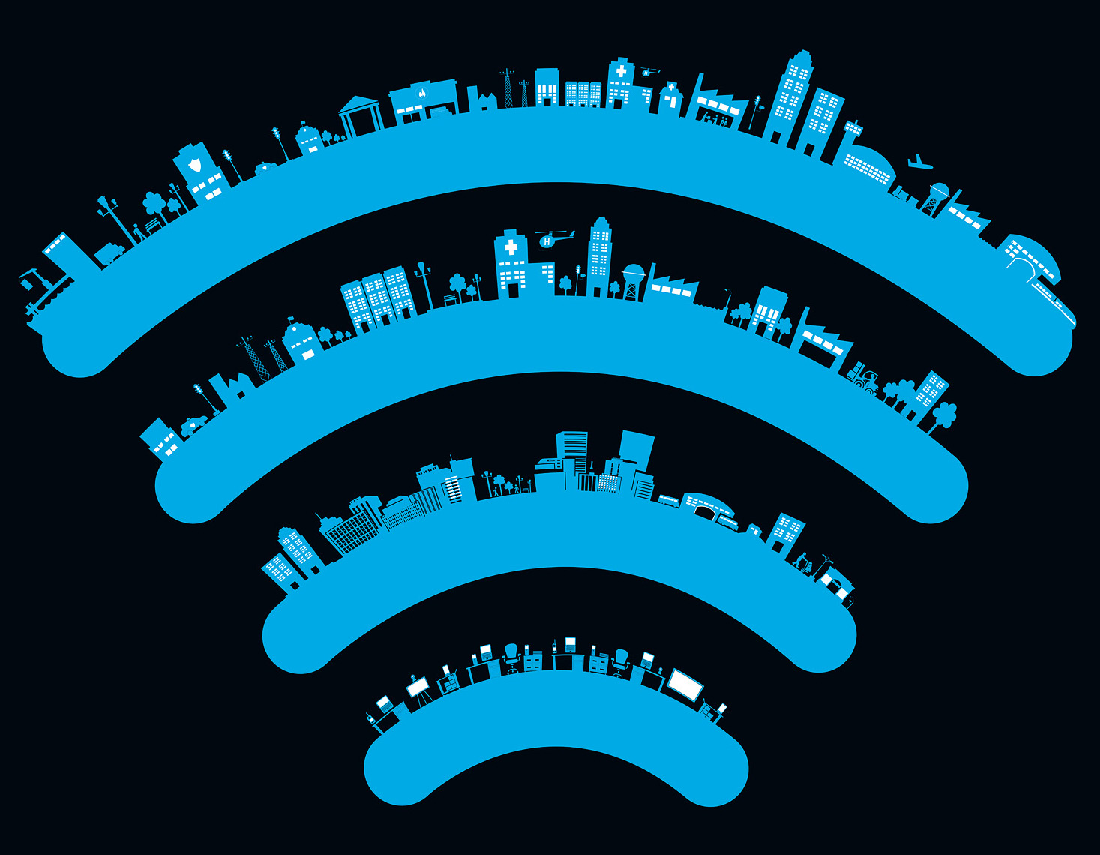
\includegraphics[width=2.0in]{MOT_WNS.pdf}
   \label{connectivity}
  \end{figure}
  \column{2in}
  \begin{figure}
    \includegraphics[width=2.0in]{connectivity.pdf}
  \label{MOT_WNS}
  \end{figure}
\end{columns}
\begin{itemize}
  \item Mobile wireless networks have enjoyed tremendous growth due to the ever-increased demands of mobile applications.
  \item Moreover, the growth is expected to continue unabated with the increasing popularity of ubiquitous smart systems.
  \item The fundamental consideration is how to get suitable trade-off between system reliability and transmission rate?
\end{itemize}
\end{frame}

\subsection{Zooming}
\begin{frame}
\frametitle{Zooming Figures}
\framezoom<1><2>[border](0.5cm,0.5cm)(2cm,1.5cm)
\pgfimage[height=6cm]{whyblue}
%
\includegraphics[height=6cm]{whyblue} is working, too!
Click the border to zoom in.
\end{frame}

\subsection{Tables}
\begin{frame}{Tables}
\begin{block}{Results}
\begin{itemize}
  \item $\Delta d$ is more larger compared to Lee's method when $K=0$, which means the multi-path fading is Rayleigh distributed.
  \item $\Delta d$ may be not so small although $2L$ decreases, for $n<5$ when the terrains gradually become flat until $\nu>10$.
\end{itemize}
\end{block}
\begin{table}[!t]
\renewcommand{\arraystretch}{1}
\centering
\begin{threeparttable}[b]
\caption{Summary of Experiment Results}
\label{summary}
\setlength{\tabcolsep}{4pt}
\scriptsize
\begin{tabular}{c|c||c|c||c|c||c|c||c|c|c}
\hline
\multicolumn{1}{c|}{\multirow{3}{*}{Terrain}} & \multicolumn{1}{c||}{\multirow{3}{*}{$K$(dB)}} & \multicolumn{1}{c|}{\multirow{3}{*}{$\nu$}} & \multicolumn{1}{c||}{\multirow{3}{*}{$\sigma$}} & \multicolumn{1}{c|}{\multirow{3}{*}{$2L(\lambda)$}} & \multicolumn{1}{c||}{\multirow{3}{*}{$N$}} & \multicolumn{1}{c|}{\multirow{3}{*}{$\Delta d(\lambda)$}} & \multicolumn{1}{c||}{\multirow{3}{*}{$\Delta d$(m)}} & \multicolumn{3}{c}{$v_{train}$(km/h)}\\
\cline{9-11}
\multicolumn{1}{c|}{} & \multicolumn{1}{c||}{} & \multicolumn{1}{c|}{} & \multicolumn{1}{c||}{} & \multicolumn{1}{c|}{} & \multicolumn{1}{c||}{} & \multicolumn{1}{c|}{} & \multicolumn{1}{c||}{} & 200 & 250 & 300\\
\cline{9-11}
\multicolumn{1}{c|}{}& \multicolumn{1}{c||}{} & \multicolumn{1}{c|}{} & \multicolumn{1}{c||}{} & \multicolumn{1}{c|}{} & \multicolumn{1}{c||}{} & \multicolumn{1}{c|}{} & \multicolumn{1}{c||}{} & \multicolumn{3}{c}{$\Delta t$(ms)}\\
\cline{1-11}
NLOS\tnote{*}  &  0 &    - & - & 40 & 36 &  1.1 & 0.367 &  2.20 &  1.76 &  1.47\\
\hline
Intensive  &  0 &    0 & 1 & 55 & 15 &  3.7 & 1.222 &  7.33 &  5.86 &  4.89\\
           &  2 &    4 & 2 & 18 & 12 &  1.5 & 0.500 &  3.00 &  2.40 &  2.00\\
           &  4 &  5.6 & 2 &  9 &  9 &  1.0 & 0.333 &  2.00 &  1.60 &  1.33\\
           &  6 &    6 & 3 & 20 &  7 &  2.9 & 0.967 &  5.80 &  4.64 &  3.87\\
           &  8 &   12 & 3 &  8 &  1 &  8.0 & 2.667 & 16.00 & 12.80 & 10.67\\
Open       & 10 &   18 & 4 & 12 &  1 & 12.0 & 4.000 & 24.00 & 19.20 & 16.00\\
\hline
\end{tabular}
\begin{tablenotes}
\item[*] \tiny Caculated by Lee's method in the case of Rayleigh fading
\end{tablenotes}
\end{threeparttable}
\end{table}
\end{frame}

\section{Equations and Codes}
\subsection{Equations}
\begin{frame}{Equations}
\begin{block}{Number of Averaging Samples}
The expectation and variance of $r^2$ can be calculated:

\begin{equation}
    \bar{r^2}=E\left[r^2\right]=\frac{1}{N}E\left[\sum_{i=1}^{N}z_i^2\right]=\frac{\sigma^2}{N}\left(2N+\nu^2\right)
\label{number_mean}
\end{equation}

\begin{equation}
    \sigma_{\bar{r^2}}=D\left[r^2\right]=\frac{1}{N^2}D\left[\sum_{i=1}^{N}z_i^2\right]=\frac{\sigma^4}{N^2}\left(4N+4\nu^2\right)
\label{number_sigma}
\end{equation}
\end{block}
\pause
\uncover<2->
{
\centering
{\Large $\Downarrow$}
\footnotesize
\begin{equation}
\begin{split}
    Q_e=10 \log_{10}\left(\frac{\bar{r^2}+\sigma_{\bar{r^2}}}{\bar{r^2}}\right)&=10 \log_{10}\left(\frac{\frac{\sigma^2}{N}\left(2N+\nu^2\right)+\frac{2\sigma^2}{N}\sqrt{N+\nu^2}}{\frac{\sigma^2}{N}(2N+\nu^2)}\right)\\
    &=10 \log_{10}\left(\frac{2N+\nu^2+2\sqrt{N+\nu^2}}{2N+\nu^2}\right)
\end{split}
\label{Q_e}
\end{equation}
}
\end{frame}

\subsection{Algorithms}
\begin{frame}{Algorithms}
\begin{algorithm}[H]
%\SetAlFnt{\footnotesize}
%\floatname{algorithm}{Procedure}
\renewcommand{\algorithmicrequire}{\textbf{Input:}}
\renewcommand{\algorithmicensure}{\textbf{Output:}}
\caption{GradedM}
\label{alg:graded}
\begin{scriptsize}
\begin{algorithmic}[1]
\Require tx-complete \Comment{packets transmitted event}
\Ensure  rate-index \Comment{rate selection index of HT/GI/MCS}
\While{$txcomplete$} \Comment{defined in \textsf{xmit.c}}
\State{update $txstatus$;}
\State{\Call {DSWA}{$pdrlast,pdrnow$}; \Comment{defined in \textsf{DSWA.c}}}
\State{$rssnow$ $\leftarrow$ \Call{Average}{$rxstatusrss$}; \Comment{defined in \textsf{recv.c}}}
\State{\Call{GradedM}{$pdrnow,rssnow$}; \Comment{defined in \textsf{GradedM.c}}}
\EndWhile
\If{$pdrnow < P_{thrh}$ or $ rssnow < \delta_+$}
\State{$gradedtalbe \gets$ \Call{GradedM}{$pdrnow,rssnow$};} \Comment{defined in \textsf{rc.c}}
\State{$rateindex \gets$ \Call{down-mcs}{$gradedtable$};}
\EndIf
\If{$gradedsens - rssnow > highlimittogray$}
\State{$rateindex \gets$ \Call{up-mcs}{$gradedtable$};}
\EndIf
\State \Return{\{$txstatus,rateindex$\};}
\Function{DSWA}{$pdrlast,pdrnow$}\label{funcDSWA}
  \State{\{$W, \beta$\} $\gets$ \Call{update}{$pdrlast,pdrnow$}}; \Comment{Equation \ref{Q_e}}
  \State{\{$\gamma, \eta$\} $\gets$ \Call{update}{$pdrlast,pdrnow,W,\beta$}; \Comment{Equation \ref{Q_e}}}
  \State{\Return{\{$W,\beta$\}};}
\EndFunction
\end{algorithmic}
\end{scriptsize}
\end{algorithm}
\end{frame}

\subsection{Codes}
\begin{frame}[fragile]
\frametitle{Codes}
The code layout follows the GNU coding standard \sfcite{GNUCoding}.
\begin{lstlisting}
#include "intelhew.h"
void IntelHew::SetHewScenario
{
  switch (scenariotype)
    {
      case RESIDENTIAL:
        StartScenarioResidential(intelHew);
        break;
      default:
        StartScenarioIndoor(intelHew);
        break;
    }
  // Scheduling the CCA only scheduler
  if (wifiMode == INTELHEW_WIFI_CCAOnly_MODE)
    {
      m_sch = CreateObject<CcaOnlyScheduler>();
      Simulator::Schedule(Seconds(0.0),
        &CcaOnlyScheduler::CcaOnlySchedulerInit, m_sch, this);
    }
}
\end{lstlisting}
\end{frame}


%\appendix

\section*{References}
\begin{frame}[allowframebreaks]{References}
  \printbibliography
\end{frame}

% All of the following is optional and typically not needed.
\section<presentation>*{}
\subsection<presentation>*{}

\section*{Q\&A}
\begin{frame}[b]{Q\&A}\label{sect:qa}
\centerline
{
  \fontsize{25pt}{10pt} \textbf{THANKS!}
}
  \vspace{1.5in}
%\centerline
%{
%  \small {\color{blue} http://yongsen.github.com}
%}
\hyperlink{outline}{\beamergotobutton{Back to Outline}}
\end{frame}

\appendix

\section*{Appendix}

\subsection*{Local Mean Power Estimation}

\begin{frame}
\frametitle{Problem Formulation}
\begin{block}{1. Propagation Model: ~~~ $p_{r}^{2}(x) = s(x)h(x)$}
\begin{enumerate}
  \item Shadowing fading:
  \begin{equation}
  s(x) \sim N\left( m(x),\sigma_s^2 \right)
  \end{equation}
  \item Multi-path fading:
  \begin{equation}
  \begin{split}
  h(x)=&\underbrace{\frac{1}{\sqrt{1+K}}\lim_{M \to \infty}\frac{1}{\sqrt M}\sum_{m=1}^{M}a_{m}e^{j\left(\frac{2\pi}{\lambda}\cos(\theta_{m}x)+\phi_m\right)}}_{\rm NLOS~Components}\\
  &+\underbrace{\sqrt{\frac{K}{1+K}}e^{j(\frac{2\pi}{\lambda}\cos(\theta_{0}x+ \phi_0))}}_{\rm LOS~Component}
  \end{split}
  \label{rician}
  \end{equation}
\end{enumerate}
\end{block}
%where $M(x)= K_1+K_2\log(x)$ and $R_{s}(x) = \sigma_{s}^2\exp\left(-\Delta x/x_0\right)$
%\begin{equation}
%    f(y;\sigma,\nu)=\frac{y}{\sigma^2}e^{-\frac{y^2+\nu^2}{2\sigma^2}}I_0\left(\frac{y\nu}{\sigma^2}\right)
%\label{ricianPDF}
%\end{equation}
\hyperlink{sect:qa}{\beamergotobutton{Back}}
\end{frame}


\end{document}


